\title{Sonart -- Der Fledermauslogger}

\team{%
    Konrad Fellmann,
    Lorenz Moser,
    Loris De Fina,
    Lukas Neuenschwander,
    André Lüscher,
    Christian Käser,
    Patrick Linggi}

\client{Meier Matthias}

\coaches{%
    Matthias Meier,
    Peter Ganzmann,
    Anita Gertiser,
    Bonnie Domenghino,
    Pascal Buchschacher}

\fssummary{
    Die meisten der rund 30 Fledermausarten in der Schweiz sind vom Aussterben
    bedroht und  Informationen über diese kleinen  flatternden Säugetiere zu
    sammeln und  zu verbreiten,  ist im Sinne  des Artenschutzes. Nur  was man
    kennt  kann  man  schützen! Da  ihre  Rufe in  einem  für  den  Menschen
    unhörbaren Bereich  liegen. wurde der  Sonart entwickelt, der  diese Rufe
    aufzeichnet und am Smartphone Grafisch und Akustisch wiedergeben kann.
}

\fsgraphics{
    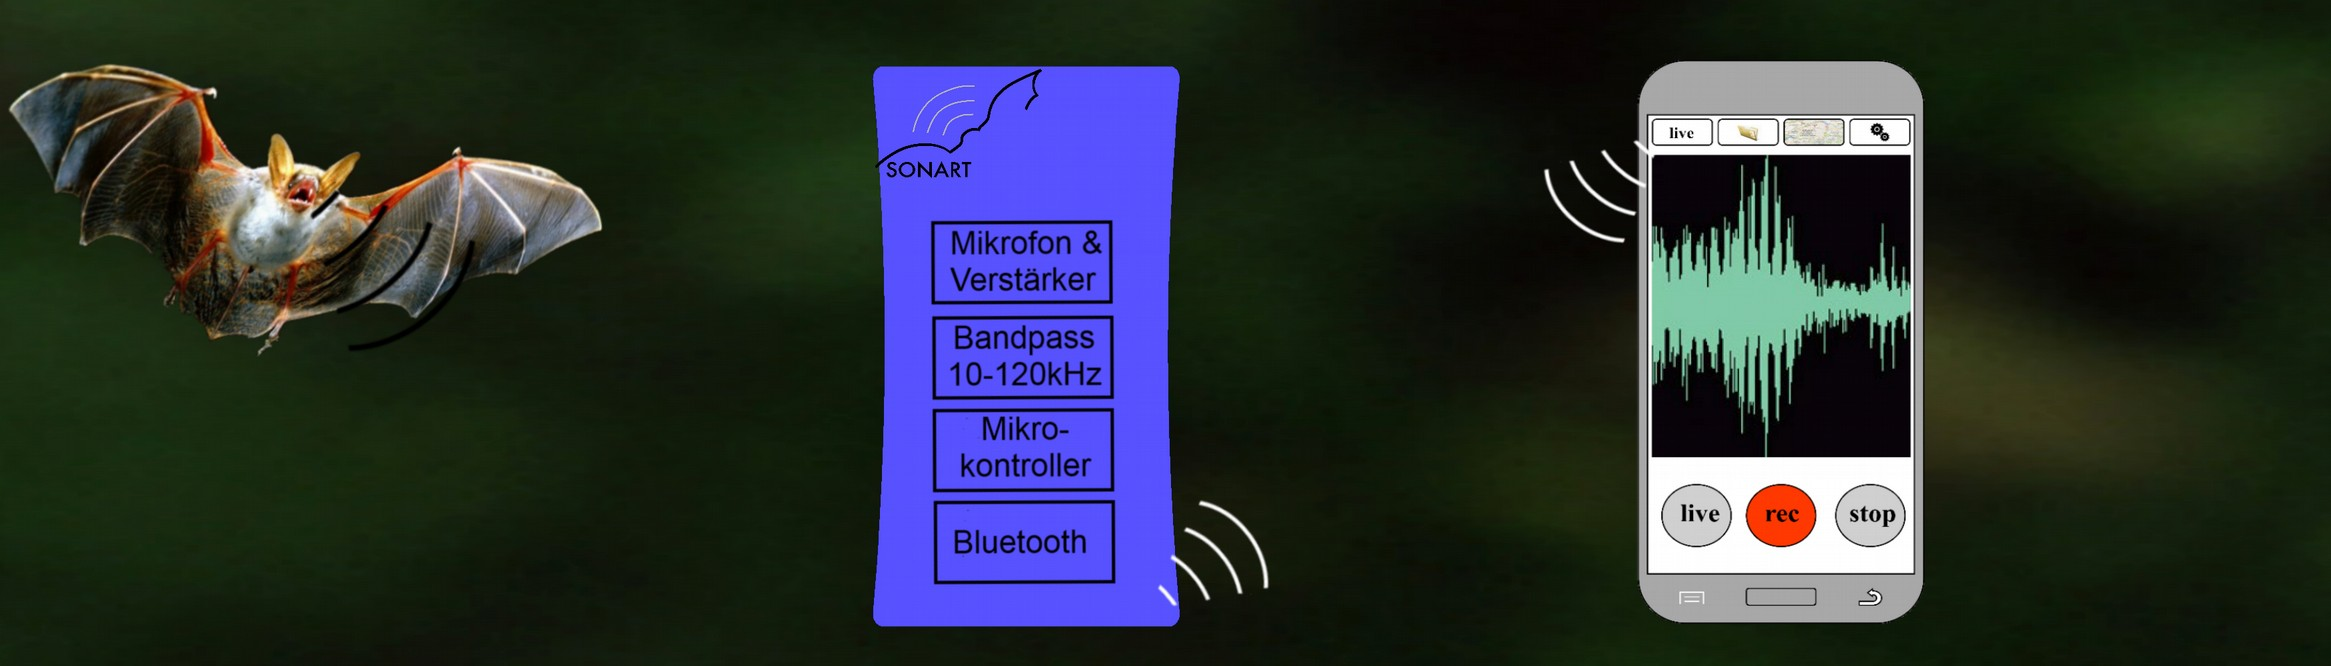
\includegraphics[width=\textwidth]{images/sonart0}
    \graphicscaption{\"Ubersicht Sonart}
    \graphicssource{lpv-augsburg.de}
}

\fscontent{
    \section{Rufe der Fledermaus}
    Die  Ortungs- und  Jagdrufe der  Fledermausarten in  der Schweiz  liegen im
    Frequenzbereich zwischen  \num{10} und \SI{120}{\kHz}, also  in einem für
    den Menschen grösstenteils unhörbaren Bereich.

    Der Ruf ändert während der Rufdauer seine Frequenz:
    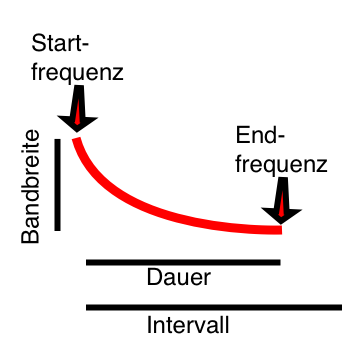
\includegraphics[width=0.9\columnwidth]{images/sonart1}
    {\footnotesize\color{parties}\textit{Quelle: }fledermausrufe.de}

    Diese Rufe  unterscheiden sich bei  jeder Fledermausart in  Bandbreite und
    Dauer. Auf diese Weise lässt sich mit Erfahrung die Art bestimmen.

    Um  die  Fledermausart identifizieren  zu  können,  müssen die  Ruflaute
    visualisiert werden. Da kommt der Sonart ins Spiel.


    \section{Anforderungen}
    F\"ur  den  Feldeinsatz  ist  ein  kompaktes  Ger\"at  von  Vorteil.   Der
    Sonart-Logger hat die Grösse einer Zigarettenschachtel.

    Die Rufe  werden mit einem speziellen  Mikrofon aufgezeichnet, verstärkt,
    gefiltert und via Bluetooth an das dazugehörige Android App gesendet.  Im
    Android  App  kann  zwischen zwei  verschiedenen  Abspiel-Modi  gewechselt
    werden (Live  Stream und die  h\"orbar gemachten Rufe).  Die  Laute werden
    als Wave-File aufgezeichnet und im Smartphone gespeichert.


    \section{Bedienung}
    An der Oberkannte neben dem  Mikrofon befindet sich der Hauptschalter; das
    GUI der App sieht wie folgt aus:

    \begin{minipage}{0.5\columnwidth}
        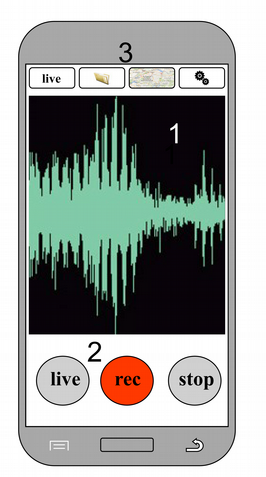
\includegraphics[width=\textwidth]{images/sonart2}
    \end{minipage}
    \begin{minipage}{0.5\columnwidth}
        \raggedright
        \begin{enumerate*}[label={\alph*)}]
            \item Darstellung der Laute
            \item Bedientasten
            \item Einstellungen
        \end{enumerate*}
    \end{minipage}
}

\infobox{Technische Daten}{%
    \begin{minipage}{0.50\textwidth}
        \setlength\leftmargini{0.5em}
        \raggedright
        \begin{itemize}\tightlist
            \item Akku: Li Ion \SI{3.7}{\volt} \SI{1100}{\milli\ampere\hour}
            \item Laufzeit: mind. \SI{10}{\hour}
            \item Gr\"osse: $\num{90} \times \num{70} \times \SI{30}{\mm^3}$
            \item Android Version 4.x
            \item Detektionsreichweite: \SIrange{0.5}{30}{\meter}
            \item Frequenzbereich: \SIrange{10}{120}{\kHz}
            \item Akku und Mikrofon sind austauschbar.
        \end{itemize}
    \end{minipage}
    \hfill
    \begin{minipage}{0.45\textwidth}
        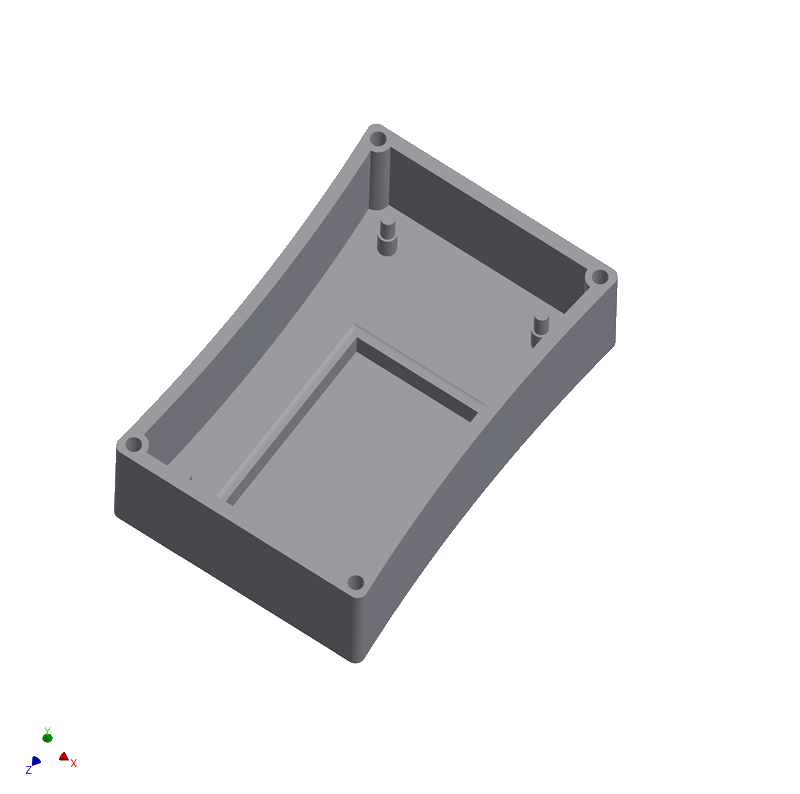
\includegraphics[width=\textwidth,clip,rviewport=0.1 0.1 0.9 0.9]{images/sonart3}
    \end{minipage}
}
